\section{Application to protoplanetary disks}\label{2dppd}
We now apply our linear framework to assess the stability of  
protoplanetary disks. We consider the gravito-turbulent disk models recently
developed by \citet[][hereafter \citetalias{rafikov15}]{rafikov15}. 
This 2D, Keplerian disk orbits a Solar 
mass star and is defined by the following parameters, 

\begin{itemize}
  \item $\dot{M}$, the global radial mass accretion rate;
  \item $Q_0$, the value of the 2D Toomre parameter where the disk is
    gravito-turbulent;
  \item $T_\mathrm{irr}$, the irradiation or floor temperature;
  \item $\alpha_m$, the dimensionless viscosity associated with other
    sources of turbulence, such as magneto-rotational instabilities
    (MRI, see also \S\ref{visc_gi} and \S\ref{MHD}). 
\end{itemize} 
These properties serve as inputs for calculating thermal equilibrium, and mass and
angular momentum conservation. Together with an opacity law, 
they allow us to construct a global disk model with surface density $\Sigma(R)$ and
temperature $T(R)$ where $R$ is the global cylindrical radius from the
star. \citepalias[See][for details.]{rafikov15} These profiles give $Q(R)$,
required for input into our linear framework. We derive other
dimensionless parameters below. 

Although our disk is global in extent, here we consider the local
stability at each radius. {\bf discuss: linear prob has no vrad in
  base state} 
%KMK I disagree with neglect of viscous flow in that there is a global Mdot. Revised version:
We are thus neglecting any global instabilities \citep{adams89,lodato05,kratter10} as well as any 
 evolution of the disk properties in response to GI.
% We are thus neglecting the slow, background viscous radial flow; as well
%as any global gravitational instabilities \citep{lodato05}. {\bf more refs?}

\subsection{Effective $\alpha$}
In a steady, viscously accreting Keplerian disk 
with constant $\dot{M}$ we have,
approximately, $\nu\Sigma = \dot{M}/3\pi$. Hence
\begin{align}
  \alpha = \frac{\dot{M}}{3\pi}\frac{\Omega(R)}{c_{s}^2(T)\Sigma(R)},  
\end{align} 
which sets the viscosity coefficient to be used at each radius. Note that the disk profiles 
employed here give constant $\dot{M}$ rather than constant $\alpha$.

\subsection{PPD beta cooling}\label{ppd_cooling}
Energy loss in \citetalias{rafikov15} is given by 
\begin{align}\label{real_cool}
  \Lambda = \frac{2\sigma}{f(\tau)}\left(T^4 - T_\mathrm{irr}^4\right)
\end{align}
per unit area, where
\begin{align}
  f(\tau) = \tau + \frac{1}{\tau}, \label{ftau} 
\end{align}
and
\begin{align}
  \tau = \kappa_d(T)\Sigma
\end{align}
is the optical depth. Recall Eq. \ref{opacity_law} 
is our opacity model where $\kappa_d\propto T^b$ with $b=2$. 
Eq. \ref{ftau} accounts for cooling in the optically-thin ($\tau\ll
1$) and optically-thick ($\tau\gg1$) regimes. 

Note that Eq. \ref{real_cool} falls within our definition of a beta cooling prescription, because
it is an explicit function of the thermodynamic states. However, we
formulated the linear problem with the standard beta cooling function 
given by Eq. \ref{beta_cool}, which has a different (less realistic) dependence on disk temperature.
 In order to adapt the existing  framework to the above PPD cooling function, we 
need to identify the equivalent $\beta$ and $\theta$ parameters that are required for the 
linearized equations (Eq. \ref{linear_beta}). 
 
%Since we are interested in the linear response of the system, the
%corresponding cooling parameters $\beta$ and $\theta$ are found by
%comparing the linearized form of the cooling function
%(Eq. \ref{real_cool}) to that of the model function
%(Eq. \ref{beta_cool}).  

%{\bf as opposed to comparing their unperturbed forms, as done in literature}
Linearizing Eq. \ref{real_cool} gives   
\begin{align}\label{linear_real_cool}
  (\gamma-1)\frac{\delta\Lambda}{\Sigma} = \frac{2\sigma(\gamma-1)
    T^4C_1}{f(\tau)c_{s}^2\Sigma}\left(\frac{\delta P}{\Sigma} -
  \frac{C_2}{C_1}c_{s}^2\frac{\delta\Sigma}{\Sigma}\right), 
\end{align}
where
\begin{align}
C_1(\tau, T) &= 4 - b\times g(\tau, T),\\ 
C_2(\tau, T) &= 4 + (1-b)\times g(\tau, T),\\ 
  g(\tau, T) &= \left( \frac{\tau^2-1}{\tau^2+1}\right)\left(1 -
  \frac{T_\mathrm{irr}^4}{T^4}\right). \label{g_def}
\end{align}
Comparing Eq. \ref{linear_real_cool} with the linearized form of the
standard cooling function, Eq. \ref{linear_beta}, we identify
\begin{align}
  &\beta = \frac{f(\tau)c_s^2\Sigma\Omega}{2\sigma(\gamma-1)C_1T^4},\label{real_beta}\\
  &\theta = \frac{C_2}{C_1},\label{real_theta} 
\end{align}
to be used in the 2D dispersion relation (Eq. \ref{thindisk}). 
Eq. \ref{real_beta} still represents a physical cooling 
time, and is consistent with previous definitions within factors of
order unity \citep[e.g.][their Eq. 2]{kratter10}.  

%KMK
However, $\theta$ is no longer a direct proxy for the irradiation level
as it was in the standard beta cooling model.
%is now an effective irradiation level. 
Eq. \ref{real_theta} shows that $\theta$ is related to the true
irradiation temperature $\tirr$ through the function $g$ given by 
Eq. \ref{g_def}, and is therefore a only a weak function of the irradiation temperature. 
A physically non-irradiated disk with $\tirr=0$ will
have a non-zero value of the `irradiation parameter', $\theta\neq0$. More specifically $\theta = O(1)$ 
for all $\tirr <T$, and for our adopted opacity law, Eq. \ref{opacity_law}, 
\begin{align*}
  \theta = \frac{4-g}{4-2g}. 
\end{align*}
Thus for $T_\mathrm{irr} = 0$ we have $5/6<\theta<3/2$ by considering
$\tau\to 0,\,\infty$. However, for $T=\tirr$ we have $\theta = 1$, as
expected intuitively.    
%%KMK 
%This results from the fact that PPD cooling generally depends on both
%$P$ and $\Sigma$, but in the absence of irradiation standard beta
%cooling only depends on $P$. 
{\bf KMK: we should discuss}

%On the
%other hand, fully irradiated disks with  $T=T_\mathrm{irr}$ have 
%$\theta=1$, as is in the previous problem formulation
%(Eq. \ref{tirr_def}). 

\subsection{Inviscid stability condition}
%We note that for our adopted opacity law, Eq. \ref{opacity_law}, 
%\begin{align*}
%  \theta = \frac{4-g}{4-2g},
%\end{align*}
%implying $5/6<\theta<3/2$. 
With our new linearized cooling function in hand, from the discussion in \S\ref{2d_inviscid} and by applying
Eq. \ref{stable_condition},  we conclude that without viscous effects 
the disk is stable everywhere if  
\begin{align} 
  \gamma > \frac{3}{2} \quad \text{and} \quad Q >
  \sqrt{\frac{6}{5}} \label{ppd_invisc_cond} 
\end{align} 
are both satisfied.  

PPDs become irradiation-dominated at large distances from the star,
where $T\to\tirr$ and $\theta\to 1$ \citep{dalessio97,kratter11}.
Then Eq. \ref{ppd_invisc_cond} relaxes to 
$\gamma,\, Q > 1$ in the outer disk. The condition on $\gamma$
is then guarenteed. On the other hand, numerical 
simulations of gravito-turbulence show that $1\lesssim Q \lesssim 2$
\citep{gammie01,rice11}, and the second inequality is generally
satisfied.   
%KMK
Taken together, this suggests that in the outer regions of a realistic
PPD, cooling %by itself may not be not responsible 
may not be the primary cause for a secondary 
instability of a gravito-turbulent disk, which might have lead to
fragmentation. This leaves viscous GI as the only possible culprit
within our framework, as we illustrate below.  

\subsection{Example 2D calculation}\label{pp2d_example}
We relax the inviscid assumption and consider a fiducial disk  model with
$\dot{M} = 10^{-6}M_\sun\,\yr^{-1}$, $Q_0=1.5$,  
$\tirr=10\mathrm{K}$, and $\alpha_m=10^{-3}$. 
%KMK
Such a high accretion rate is consistent with those expected for 
young protostellar disks \citep{shu77,enoch09}. Similarly,
$10\mathrm{K}$ is a conservatively low background irradiation level
consistent with cloud temperatures in star forming regions
\citep{plume97,johnstone01}. 
Stellar irradiation will typically elevate $\tirr$ in addition to
adding a radial dependence \citep{kratter08} 
We adopt the opacity scale $\kappa_{d0} =
5\times10^{-4}\mathrm{cm}^2\,\mathrm{g}^{-1}\,\mathrm{K}^{-2}$  as in
\citetalias{rafikov15}. We use $\gamma=1.6$, approximately applicable
to an ideal molecular gas at low temperatures 
%KMK this is just true...and used by other authors
%\citep{rice11,baehr15}. 
This choice of $\gamma$ satisfies the global inviscid stability condition
(Eq. \ref{ppd_invisc_cond}). %which simplifies the problem
%for outer disk choice of gamma doesn't matter 
%avoid complications from over-stable thermal modes 
Fig. \ref{rafikov_model} shows the equilibrium 
disk profile in terms of $Q$, $\alpha$, $\beta$, and $\theta$.  
These profiles serve as input to the 2D dispersion relation
(Eq. \ref{thindisk}, Eq. \ref{bigA}---\ref{bigF}). 

Fig. \ref{rafikov_growth} shows growth timescales and
optimum wavenumbers for viscous GI in this fiducial model. For
comparison we also plot a case with lower accretion rate, 
$\dot{M}=10^{-7}M_\sun\,\yr^{-1}$; and analytic estimates based on
Eq. \ref{gammie_smallk} (instead of Eq. \ref{gammie_maxrate_simple}
since here $\theta\sim 1$) which gives the optimum wavenumber and
growth rates as 
\begin{align}
  |K| = \frac{3}{2\theta Q}, \quad
%\end{align}
%with growth rate
%\begin{align} 
  S = \frac{27\alpha}{16\theta^3Q^4}. 
\end{align}
These are similar to the isothermal results of
\citet[][their Eq. 19 and 21, respectively]{sterzik95}, and identical if one
takes $\theta=1$. %showing that irradiation makes the disk behave like
                  %isothermal disk
 
The most unstable wavelength is a few times the disk thickness. 
%KMK
So long as $H\ll R$, this result is consistent with our use of the
local approximation. For our fiducial disk, $H/R \sim 0.07$ around 
$R\sim 100$AU, and $H/R <0.25$ througout the disk. 
The increase in $|K|$ from 
$\sim 10\mathrm{AU}$ to $\sim 20\mathrm{AU}$ is due to the decrease in
$Q$, while that from $\sim 
60\mathrm{AU}$ to $\sim 100\mathrm{AU}$ occurs as the disk transitions
from the 
optically-thick to optically-thin regime. The mismatch between the
numerical and analytic solutions at large
distances is expected since the above expressions assume $|K|\ll
1$. Nevertheless the analytic estimates reproduce qualitatively correct
behavior. 

The fiducial disk is subject to viscous GI on dynamical timescales
($\lesssim 10$ orbits) for $R\gtrsim60$AU. We note this transition
radius is also implied by Eq. 16 in \cite{kratter10}. Coincidentally,
beyond this radius $\alpha\gtrsim 0.1$ and $\beta\lesssim 3$, which is
often quoted as criteria for disk fragmentation  
\citepalias[e.g.][]{rafikov15}. Thus viscous GI may be responsible for 
the transition between gravito-turbulence and fragmentation due to the
removal of rotational support by viscous (turbulent) stresses. 

On the other hand, the lower $\dot{M}$ model also attain $\tcool\lesssim
3\Omega^{-1}$ beyond $\sim 60$AU, but $\alpha\lesssim 0.03$
everywhere. 
Applying empirical conditions for fragmentation may then lead to
contradiction. Instead, if viscosity is the physical cause for
fragmentation, then our result suggest the lower $\dot{M}$ disk should
not fragment (at least much less likely than our fiducial case) 
because the instability cannot develop on orbital timescales. 

\begin{figure}
  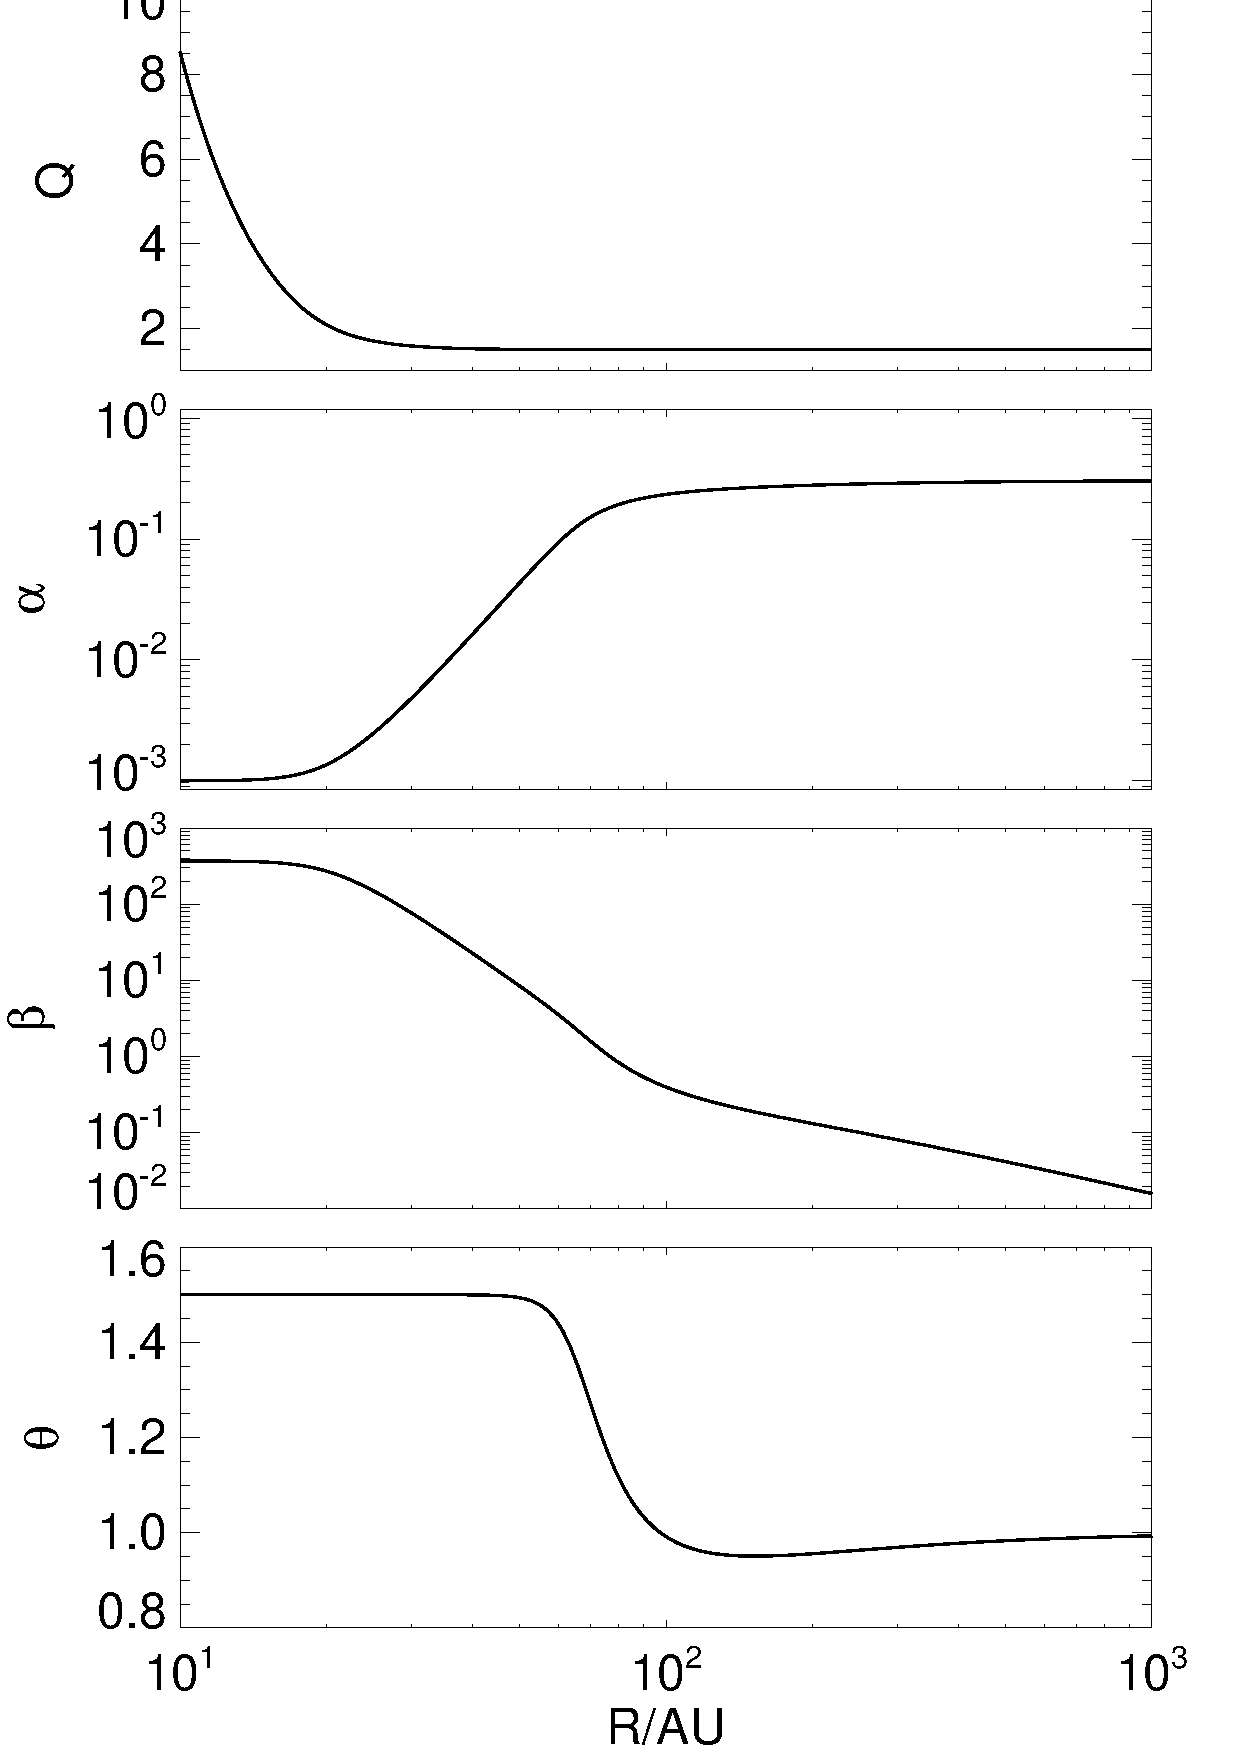
\includegraphics[width=\linewidth,clip=true,trim=0cm 0cm 0cm
    0.0cm]{figures/ppd_2d_basic}
  \caption{Equilibrium profile obtained from the disk model developed
    by \cite{rafikov15}, with parameters $\dot{M} =
    10^{-6}M_\sun\yr^{-1}$, $Q_0=1.5$, $\tirr=10\mathrm{K}$, and
    $\alpha_m=10^{-3}$.   
    \label{rafikov_model}}
\end{figure}

\begin{figure}
  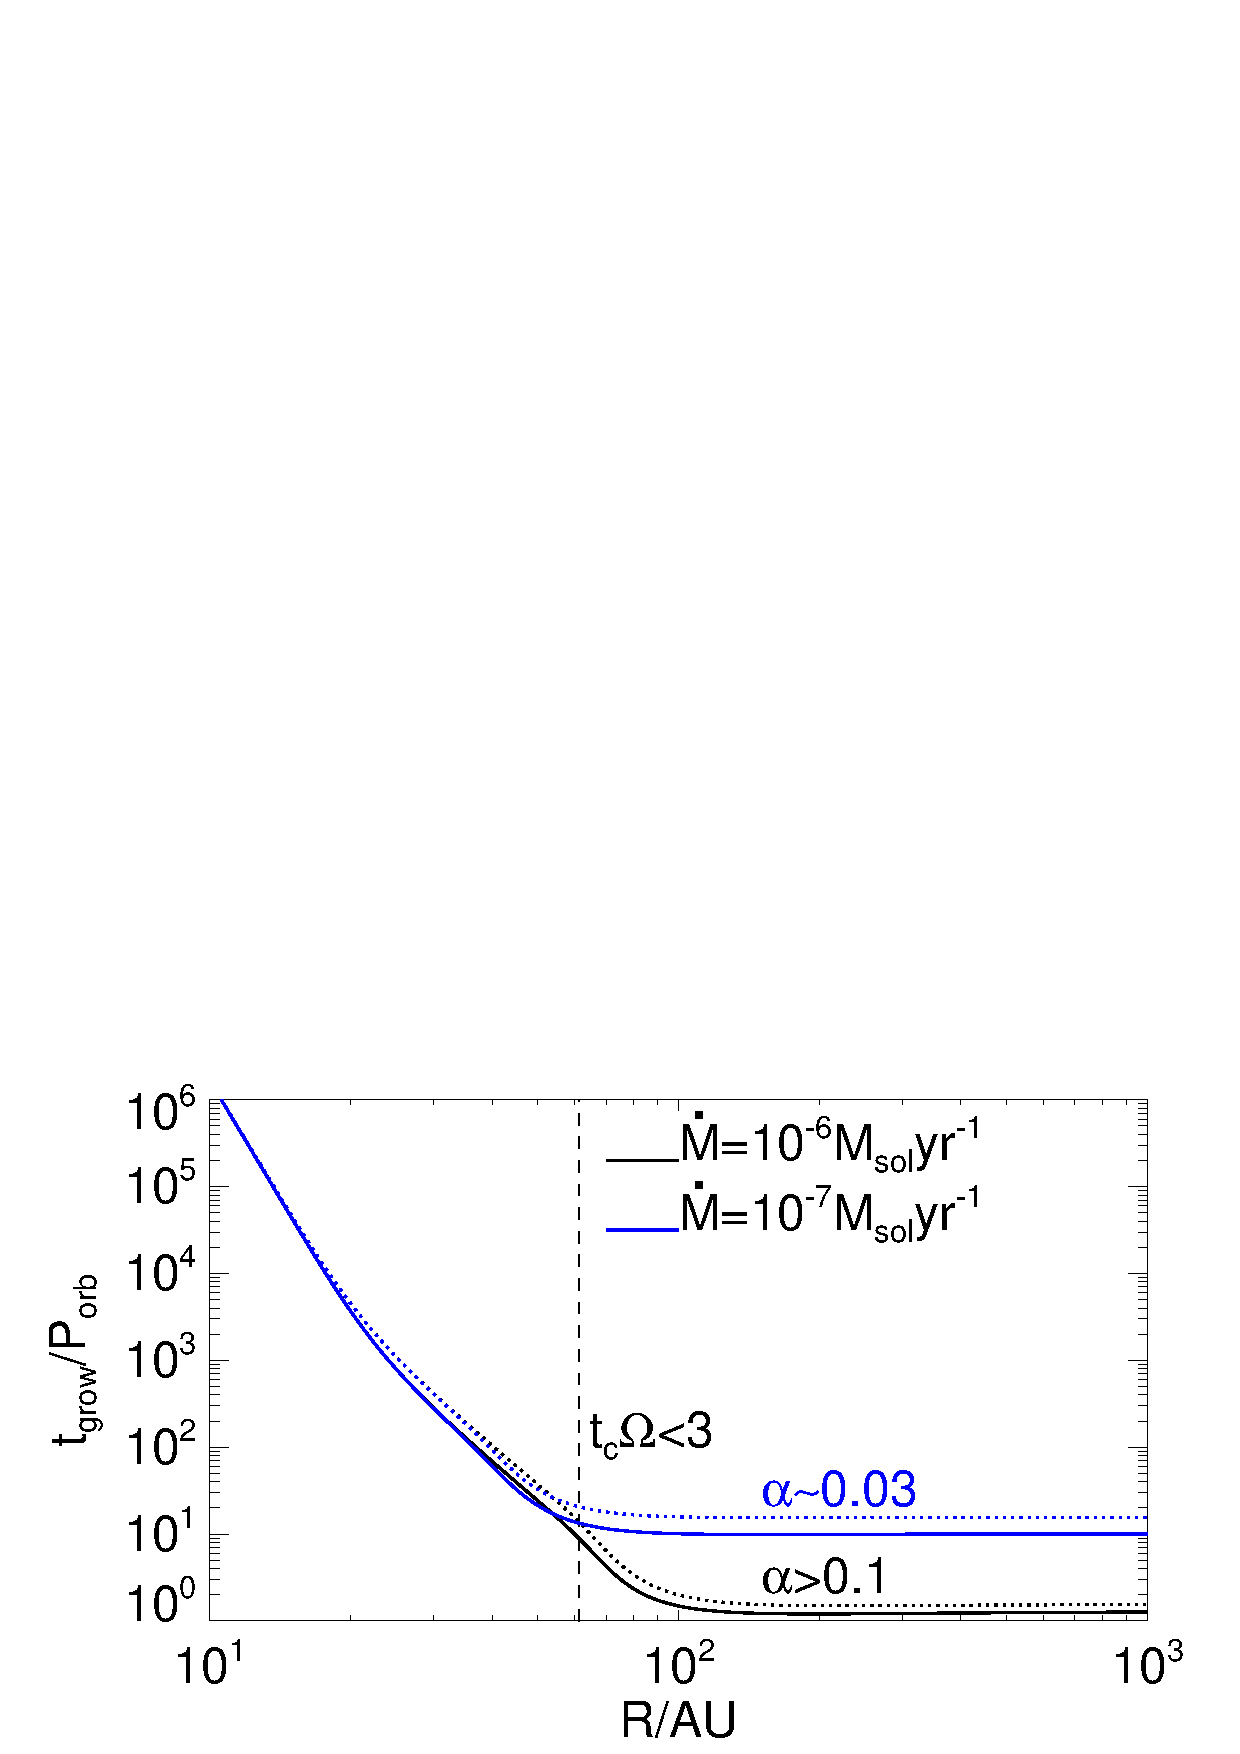
\includegraphics[width=\linewidth,clip=true,trim=0cm 2cm 0cm
    0.0cm]{figures/ppd_2d_growth}\\
  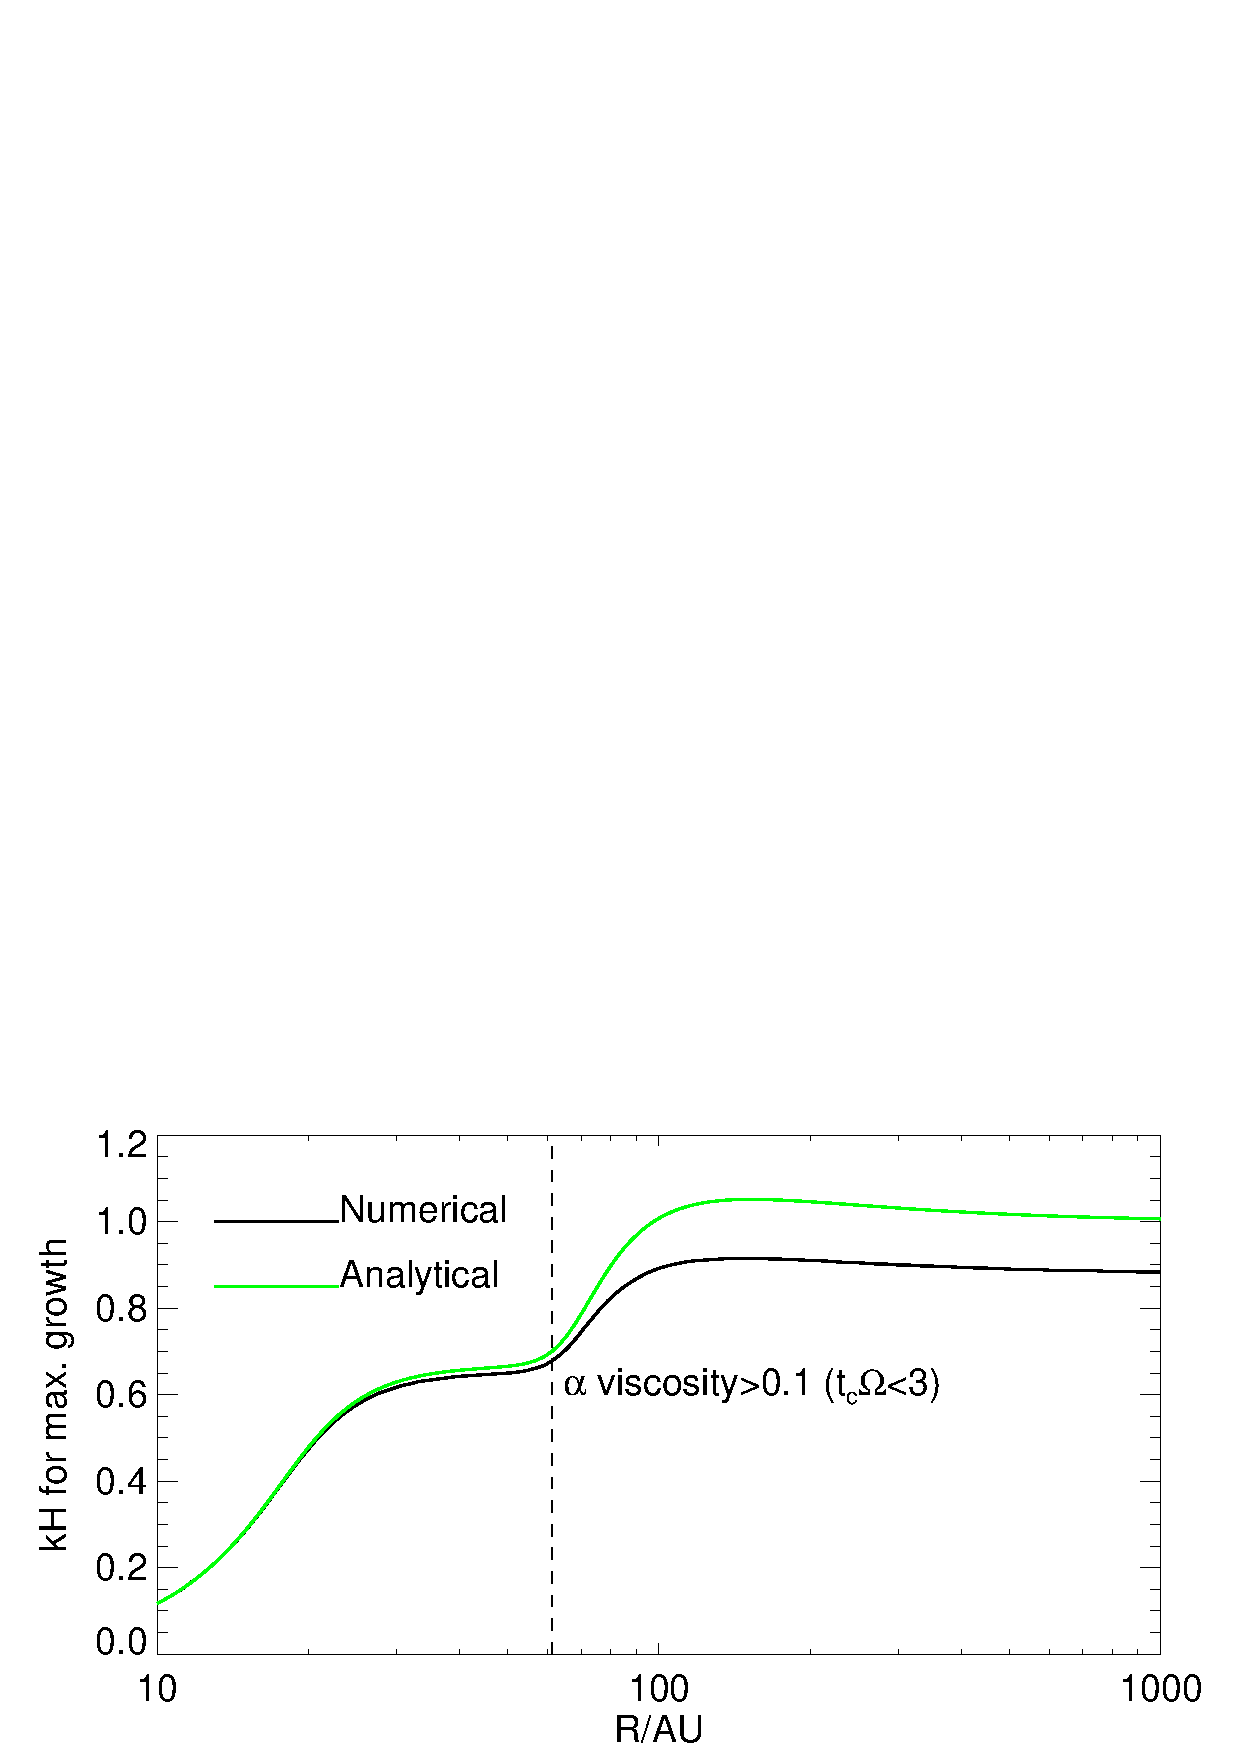
\includegraphics[width=\linewidth,clip=true,trim=0cm 0cm 0cm
    0.cm]{figures/ppd_2d_maxk}
  \caption{Black lines show growth timescales (top) of the most
    unstable wavenumber (bottom) for viscous, 
    self-gravitational modes in the 2D PPD model shown in
    Fig. \ref{rafikov_model}. Blue curves are for the same disk
    model but with a lower accretion rate. Solid curves are obtained
    numerically from Eq. \ref{thindisk}, and dotted curves 
    are analytic results based on Eq. \ref{gammie_smallk}. 
    \label{rafikov_growth}}
\end{figure}

\subsection{3D PPD with radiative diffusion}
%appropriate for not-so-large distances where irrad can be neglected 
We briefly consider 3D PPDs with explicit radiative diffusion
(\S\ref{rad_cool}). 
Given the $\alpha(R)$ and $Q(R)$ profiles obtained
from the 2D model above, at each radius $R$ we obtain the vertical
structure from Eq. \ref{vert_eq1}---\ref{thermal_eq}, with 
Eq. \ref{rad_cool1}---\ref{rad_cool2} for the radiative flux.
We then solve the 3D eigenvalue problem as in \S\ref{3ddisk}, with the
additional boundary condition that the disk surface temperature is
fixed, $\delta T(\zmax) = 0$. 
We use the fiducial disk model as in \S\ref{pp2d_example} but 
with $T_\mathrm{irr}=0$, since our simple radiative diffusion
treatment does not include irradiation (\S\ref{rad_cool}). %This also
                                %limits us 
%to smaller radii than before.  
%physically, irrad is negligible for opt thick regions, and we are
%restricted to such regions if applying rad diff
We use a slightly smaller vertical
domain with $\rho(\zmax)=0.1\rho_0$.  %to avoid very low density 

Fig. \ref{rafikov_growth3d} shows the growth rates and most unstable 
wavenumber for $R\in[10,100]$AU; along with the corresponding 2D 
results matched with softened self-gravity. There is good agreeement for
$R\lesssim60$AU where the disk is optically thick ($\tau\gtrsim
1$) and thus both models apply. However, beyond $60$AU where the disk
becomes optically-thin, radiative diffusion (the 3D curve) is not
valid and under-estimates the growth rates. %; while the $f(\tau)$
%function approximately captures opticall-thin cooling in the 2D case.  
Nevertheless, the transition radius of  
$\sim60$AU, beyond which growth timescales become dynamical,    
can be correctly calculated within the 2D framework.  
%notice the small softenings used 
%This is not surprising since the
%instability is fundamentally driven by viscous and self-gravity forces in the
%momentum equations, not the energy equation. 

\begin{figure}
  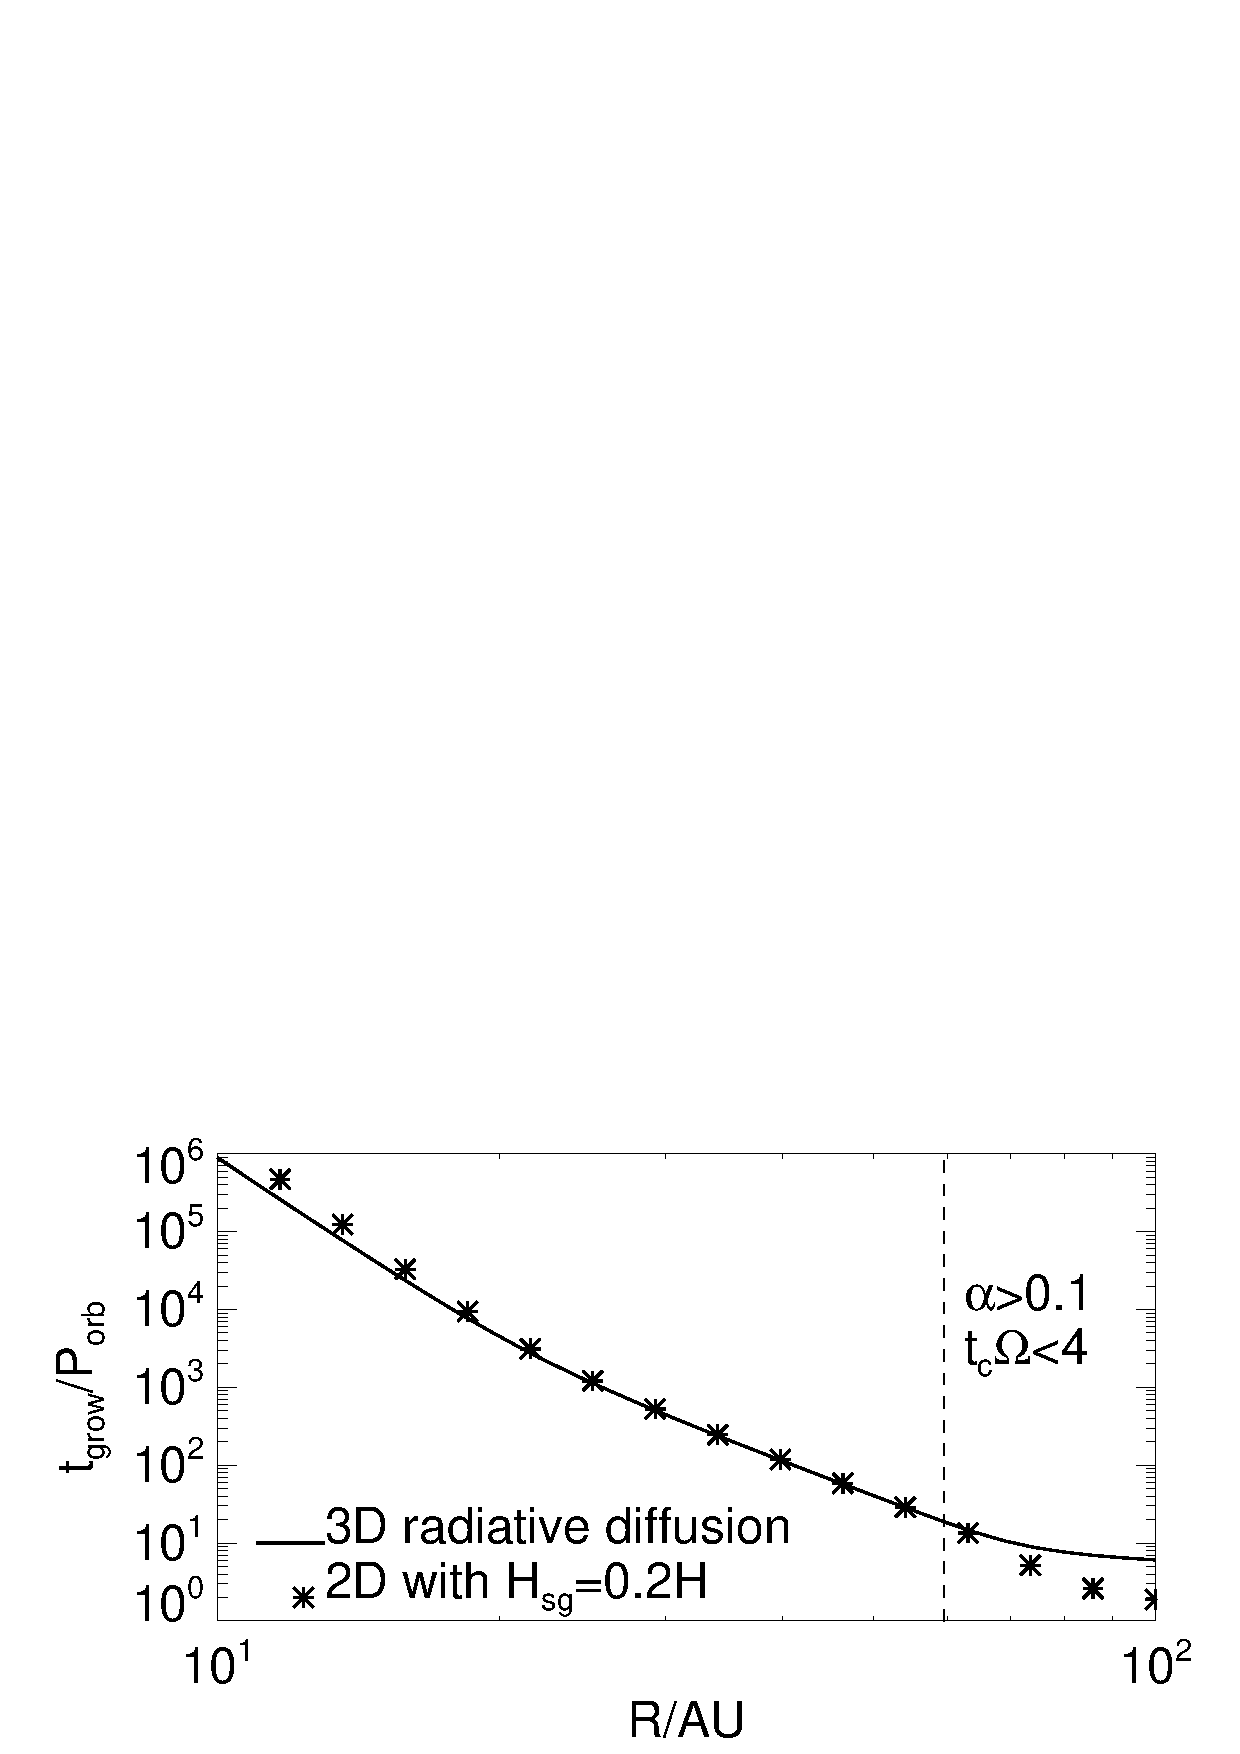
\includegraphics[width=\linewidth,clip=true,trim=0cm 2cm 0cm
    0.0cm]{figures/ppd_3d_rates}\\
  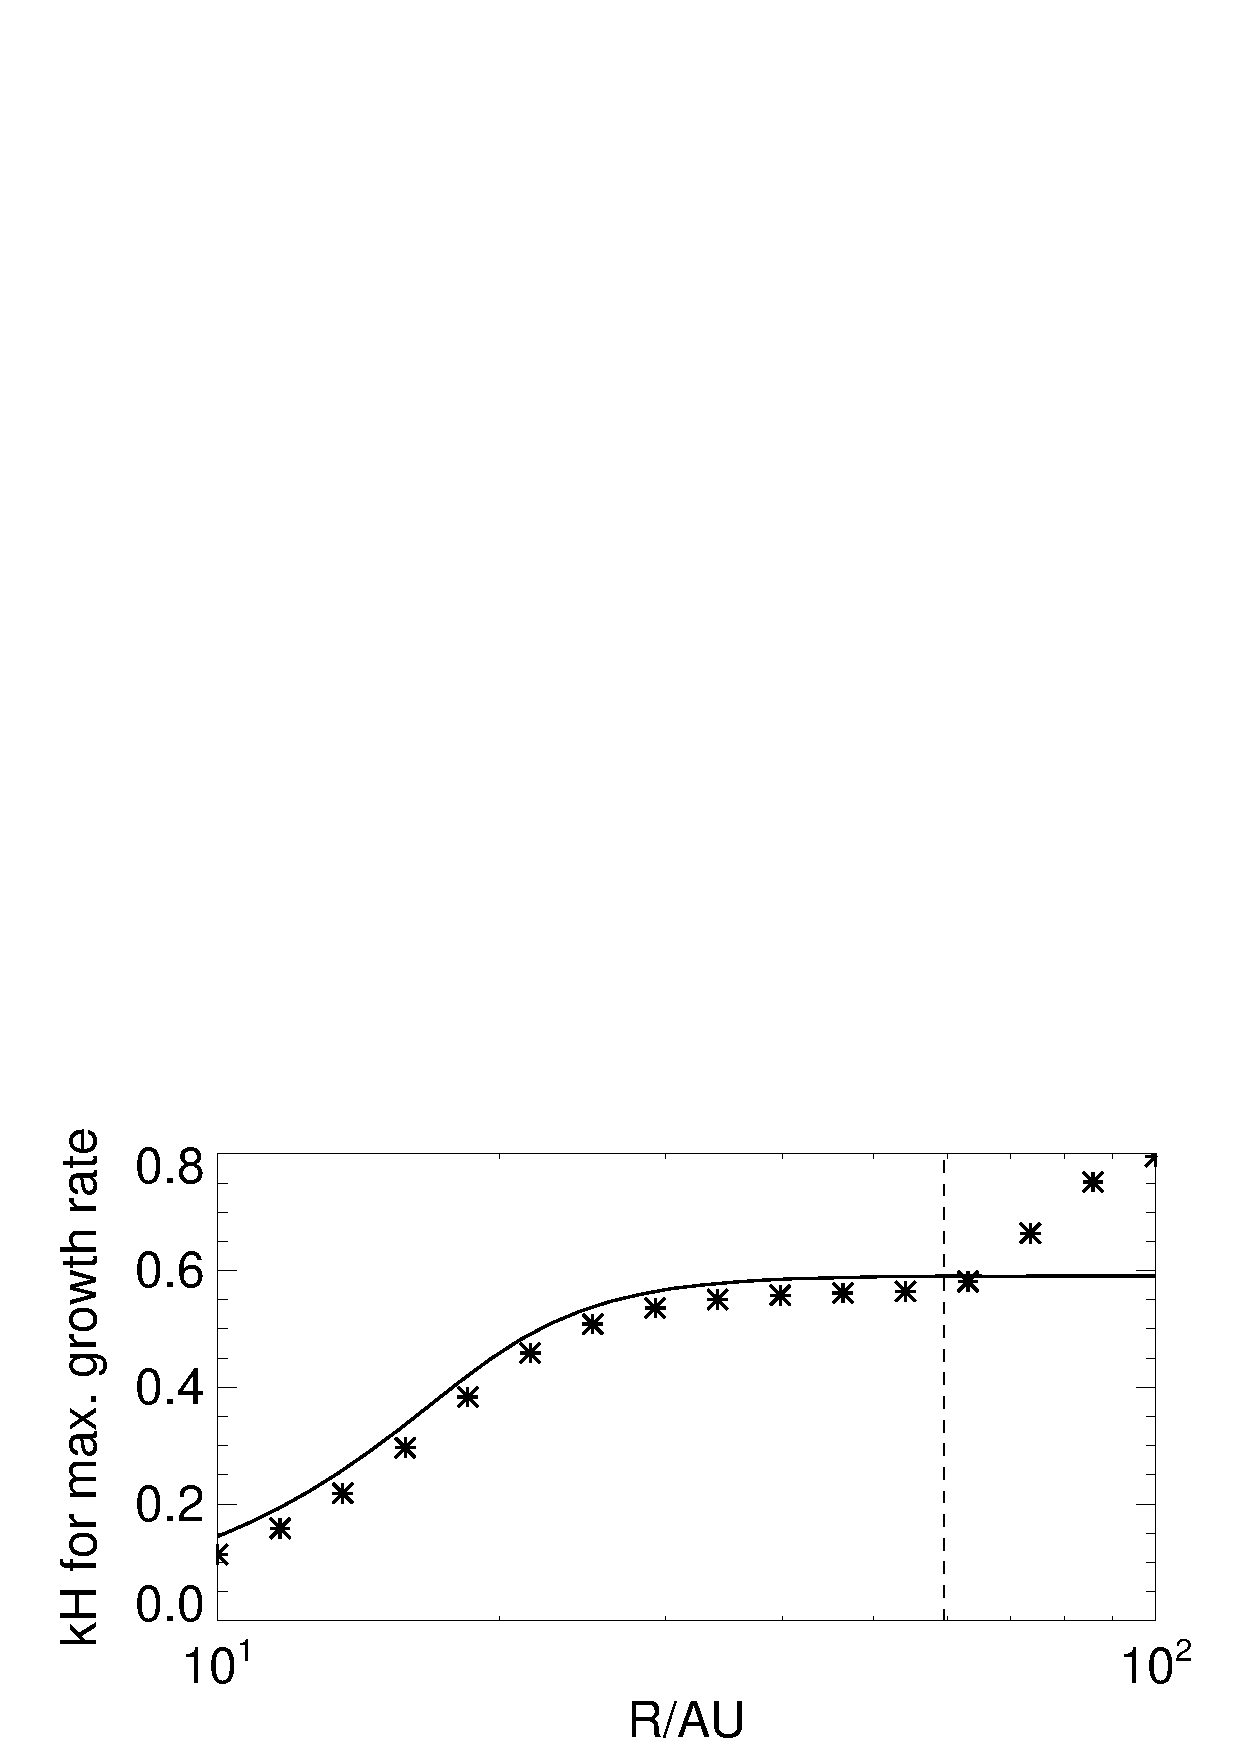
\includegraphics[width=\linewidth,clip=true,trim=0cm 0cm 0cm
    0.8cm]{figures/ppd_3d_maxk}
  \caption{Growth timescales (top) of the most unstable
    wavenumber (bottom) for viscous GI in a 3D PPD with radiative
    diffusion  (black lines). Asterisks are corresponding results
    obtained from the corresponding 2D problem with softened gravity.   
    % The black curves are obtained
  %  from the 3D eigenvalue problem with radiative diffusion,
   % applicable to optically-thick regions ($R\lesssim 60$AU); 
   % while the green curves are obtained from the 2D corresponding
   % model, which is applicable to both optically-thick and
   % optically-thin regimes.  
    \label{rafikov_growth3d}}
\end{figure}



